\documentclass[serif,xcolor=pdftex,dvipsnames,table,hyperref={bookmarks=false,breaklinks}]{beamer}

%%%%%%%%%%%%%%%%
% Change the macros below to configure the title slides
% for your course.
\newcommand{\coursename}{COMPSCI 589}
\newcommand{\instructor}{Benjamin M. Marlin}
\newcommand{\university}{University of Massachusetts Amherst}
\newcommand{\department}{College of Information and Computer Sciences}
%%%%%%%%%%%%%%%%


\newcommand{\settitlecard}[2]{
  \title[\coursename  Lecture #1] 
    {\coursename \\ Lecture #1: #2}
     \author[\instructor]{\instructor}
     \institute[\university]{
     \department\\
     \university
   }
\date{}
}

\newcommand{\maketitlepage}{
  \begin{frame}
  \titlepage
  \center{
    %If you use the slides unmodified, retain the attribution below
    \tiny{Slides by Benjamin M. Marlin (marlin@cs.umass.edu). \\
    \vspace{-1em}Created with support from National Science Foundation Award\# IIS-1350522. 
    %If you modify the slides, please retain the alternate attribution below
    %\tiny{Based on slides by Benjamin M. Marlin (marlin@cs.umass.edu). \\    
    %\vspace{-1em}Created with support from National Science Foundation Award\# IIS-1350522. 
    }                                              
  }  
  \end{frame}
}

\AtBeginSection[]
{
  \begin{frame}<beamer>{Outline}
    \tableofcontents[currentsection,subsectionstyle=hide]
  \end{frame}
}


\newcommand{\cut}[1]{}

\newcommand{\iconbox}[4]{
  \only<#1-#2>{
    \begin{columns}[T]
      \column{0.5in}
           \includegraphics[width=0.5in]{#3}
       \column{3.7in}
            #4
    \end{columns}
    \medskip
    \medskip
    \medskip
  }
}

\mode<presentation>{
  \usepackage{../beamertheme589theme}
  \setbeamercovered{invisible}
}

\mode<handout>{
  \usepackage{../beamertheme589theme}
  \setbeamercovered{transparent}
}


\usepackage[english]{babel}
\usepackage[latin1]{inputenc}
\usepackage{times}
\usepackage[T1]{fontenc}
\usepackage{amsmath}
\usepackage{amssymb}
\usepackage[noend]{algorithmic}
\usepackage{algorithm}
\usepackage{listings}

\renewcommand\mathfamilydefault{\rmdefault}

\newcommand{\setA}{\mathcal{A}}
\newcommand{\setB}{\mathcal{B}}
\newcommand{\setS}{\mathcal{S}}
\newcommand{\setV}{\mathcal{V}}
\DeclareMathOperator*{\union}{\bigcup}
\DeclareMathOperator*{\intersection}{\bigcap}
\DeclareMathOperator*{\Val}{Val}
\newcommand{\mbf}[1]{{\mathbf{#1}}}
\DeclareMathOperator*{\argmax}{arg\,max}
\DeclareMathOperator*{\argmin}{arg\,min}
\DeclareMathOperator*{\sign}{sign}
\newcommand{\deriv}[2]{\frac{\partial{#1}}{\partial{#2}}}


\settitlecard{15}{Hierarchical Clustering}

\begin{document}

\maketitlepage

\section{Introduction}
\subsection{Foo}

\begin{frame}[t]{Views on Machine Learning}

\iconbox{1}{}{../Figures/mitchell.jpg}{\textbf{Mitchell (1997):} ``A computer 
program is said to learn from experience E with respect to some class of tasks 
T 
and performance measure P, if its performance at tasks in T, as measured by P, 
improves with experience E.''\\[12pt]  Substitute ``training data D'' for  
``experience E.''}

\end{frame}

\begin{frame}[t]{Machine Learning Tasks}
 \centering
 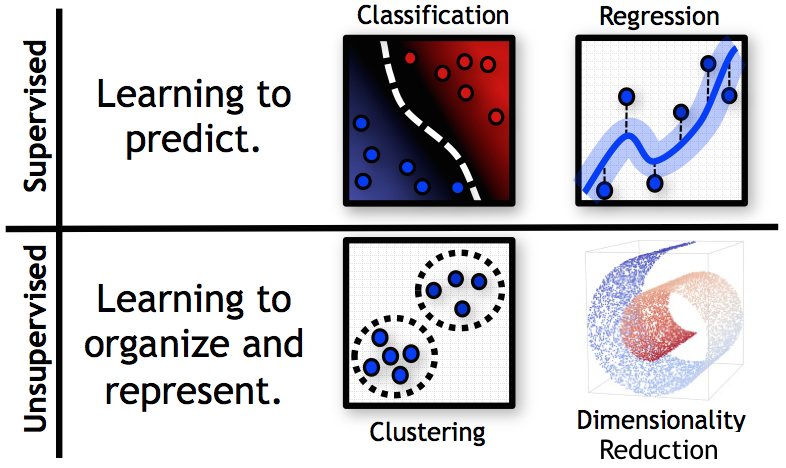
\includegraphics[width=4in]{../Figures/learning_problems.png}
\end{frame}

\begin{frame}[t]{The Classification Task}

\begin{block}{Definition: The Classification Task}
Given a feature vector $\mbf{x}\in\mathbb{R}^D$ that describes an object that 
belongs to one of $C$ classes from the set $\mathcal{Y}$, predict which class 
the object belongs to.
\end{block}

\end{frame}

\begin{frame}[t]{The Clustering Task}

\begin{block}{Definition: The Clustering Task}
Given a collection of data cases $\mbf{x}_i\in\mathbb{R}^D$, partition the 
data cases into groups such that the data cases within each partition are
more similar to each other than they are to data cases in other partitions.
\end{block}

\pause
\center
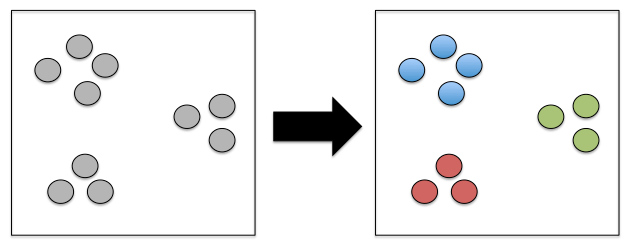
\includegraphics[width=3in]{../Figures/clustering_example.png}
\end{frame}

\begin{frame}[t]{Examples: Market Segmentation}
\center
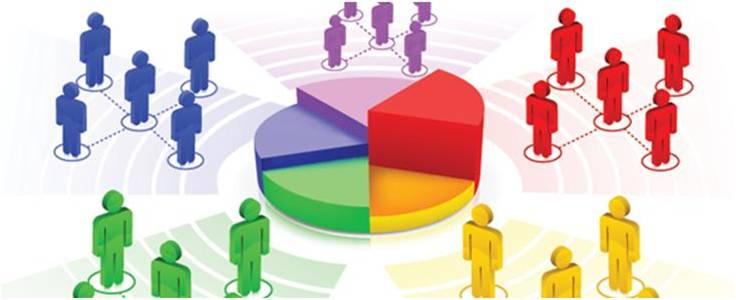
\includegraphics[width=4.5in]{../Figures/market_segmentation.jpg}
\end{frame}

\begin{frame}[t]{Examples: Community Detection}
\center
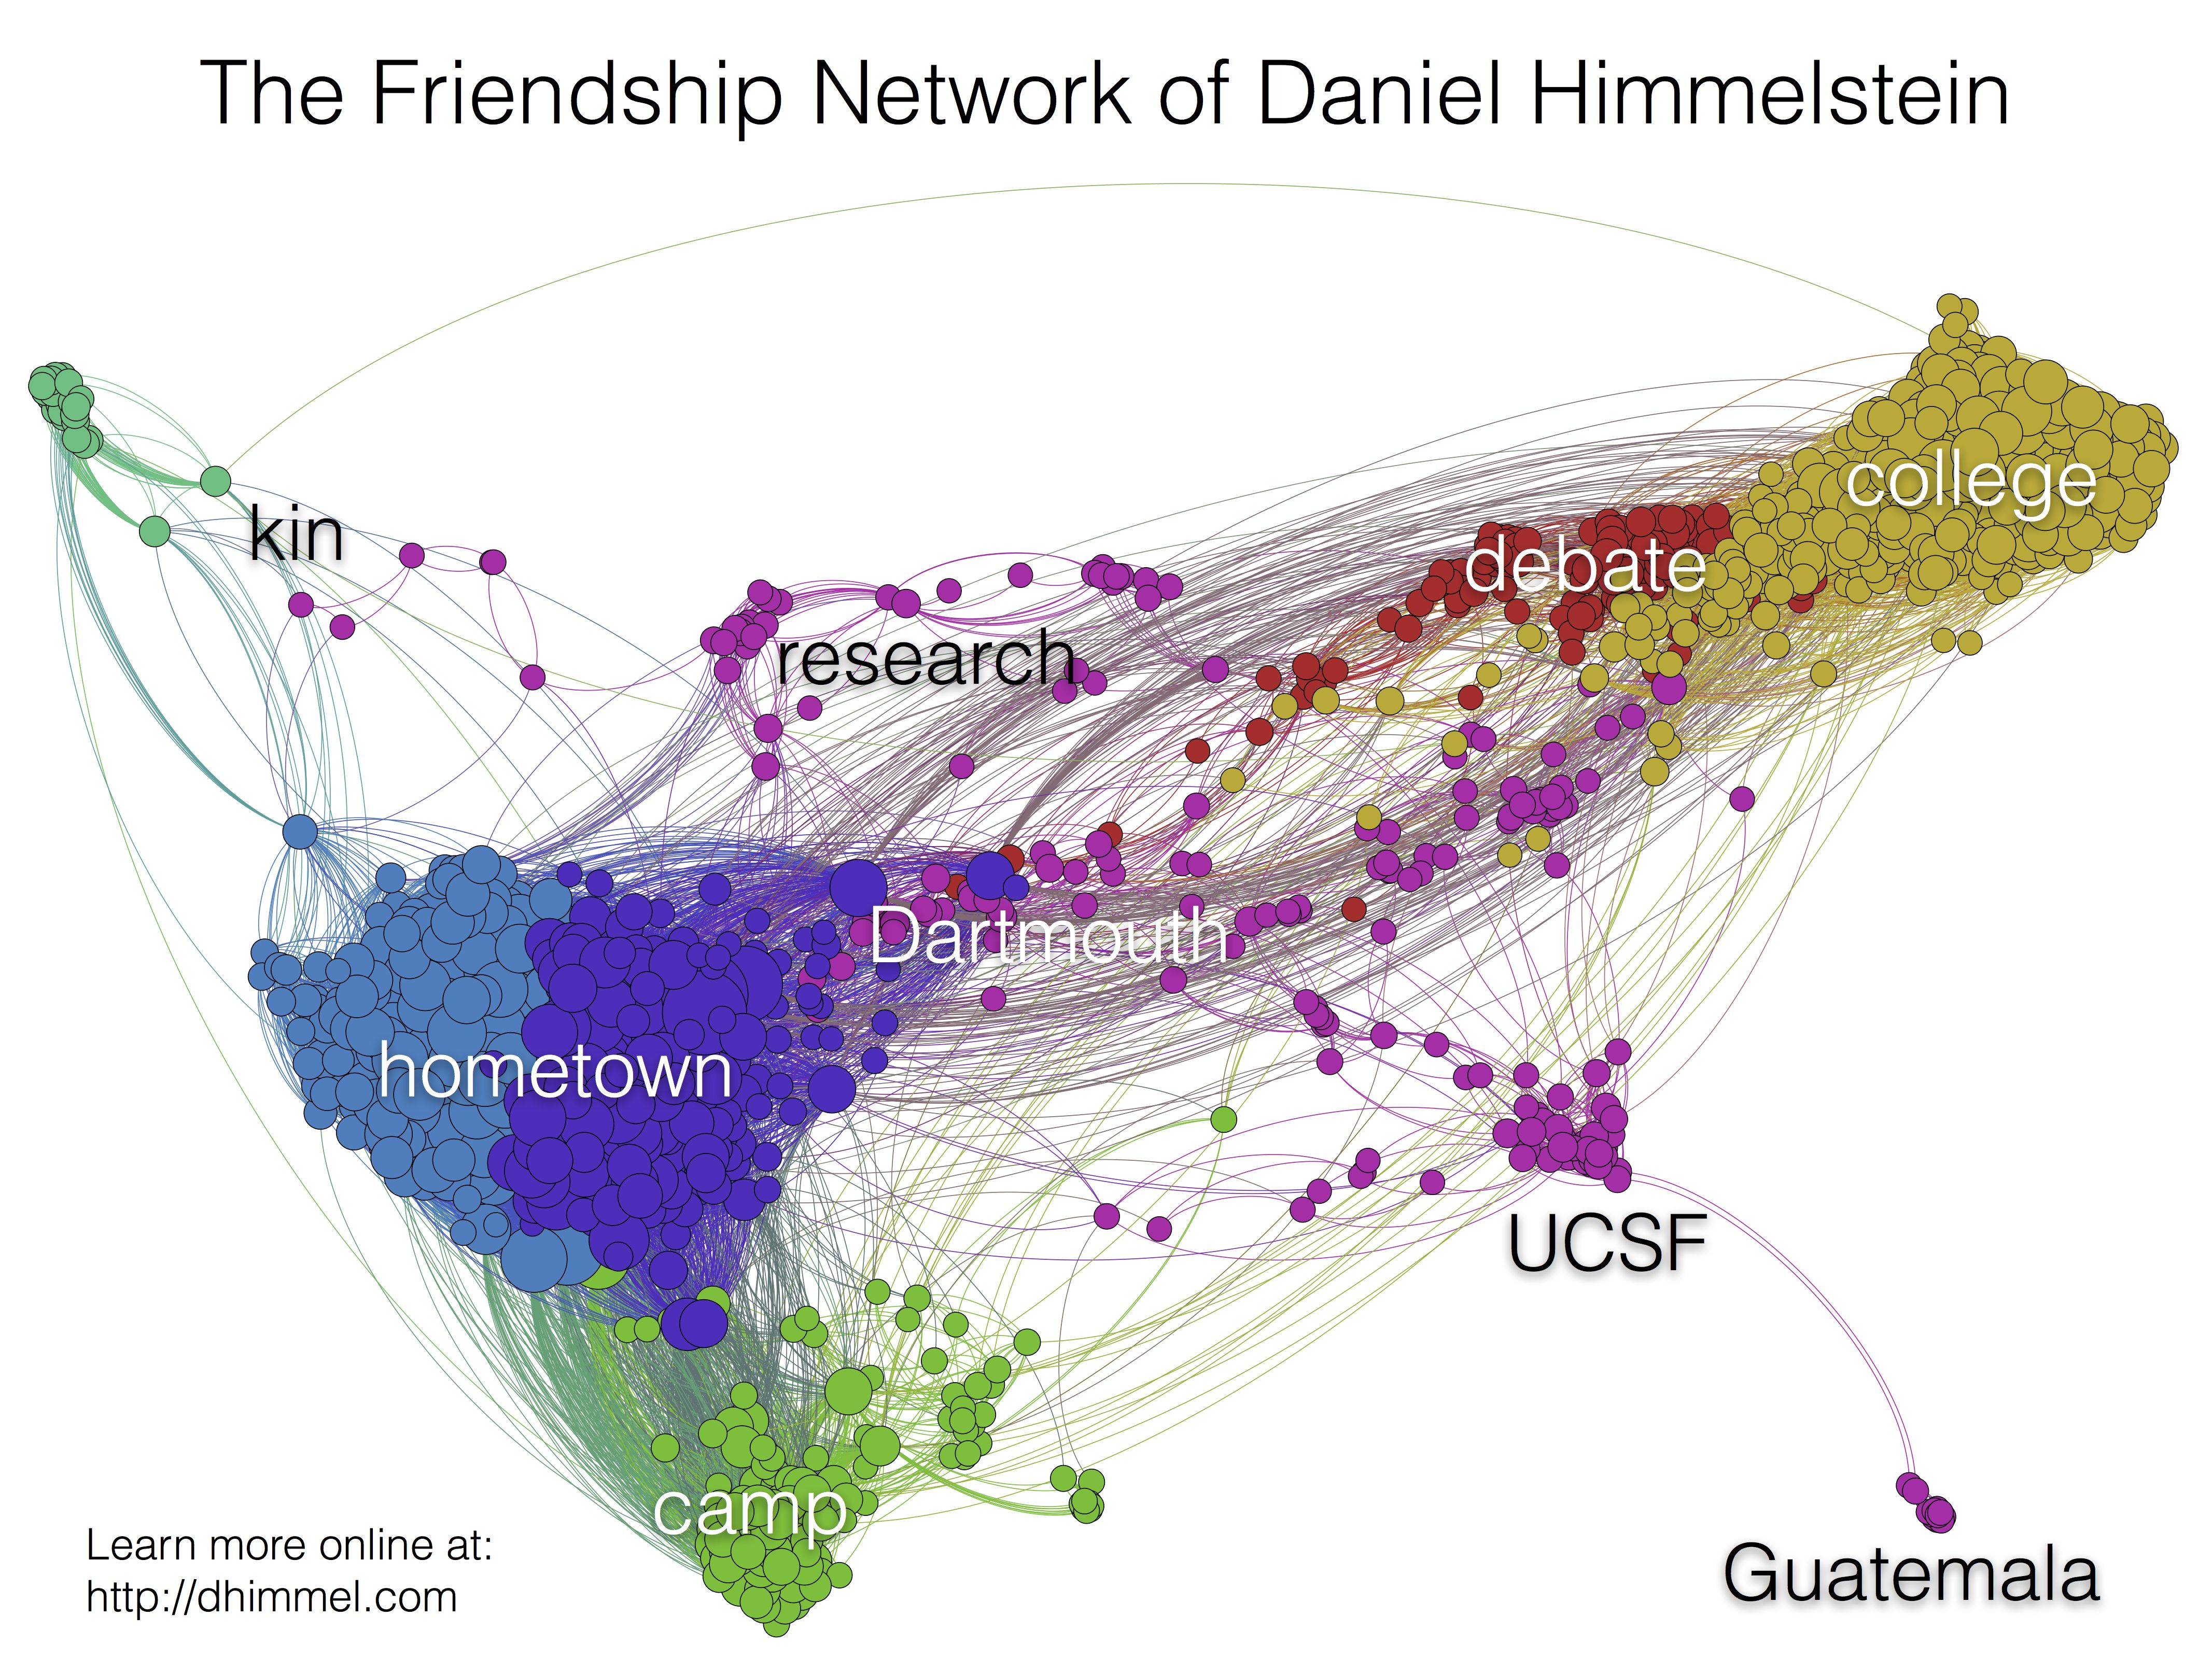
\includegraphics[width=3.5in]{../Figures/community_detection.jpg}
\end{frame}

\begin{frame}[t]{Examples: Gene Expression}
\center
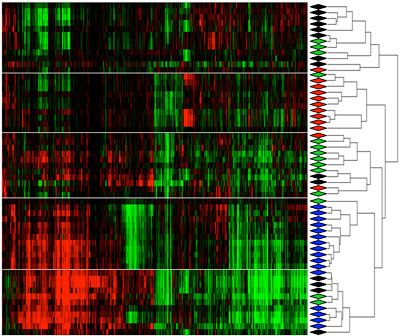
\includegraphics[width=3.5in]{../Figures/gene_clustering.jpg}
\end{frame}

\begin{frame}[t]{Examples: Phylogenetic Trees}
\center
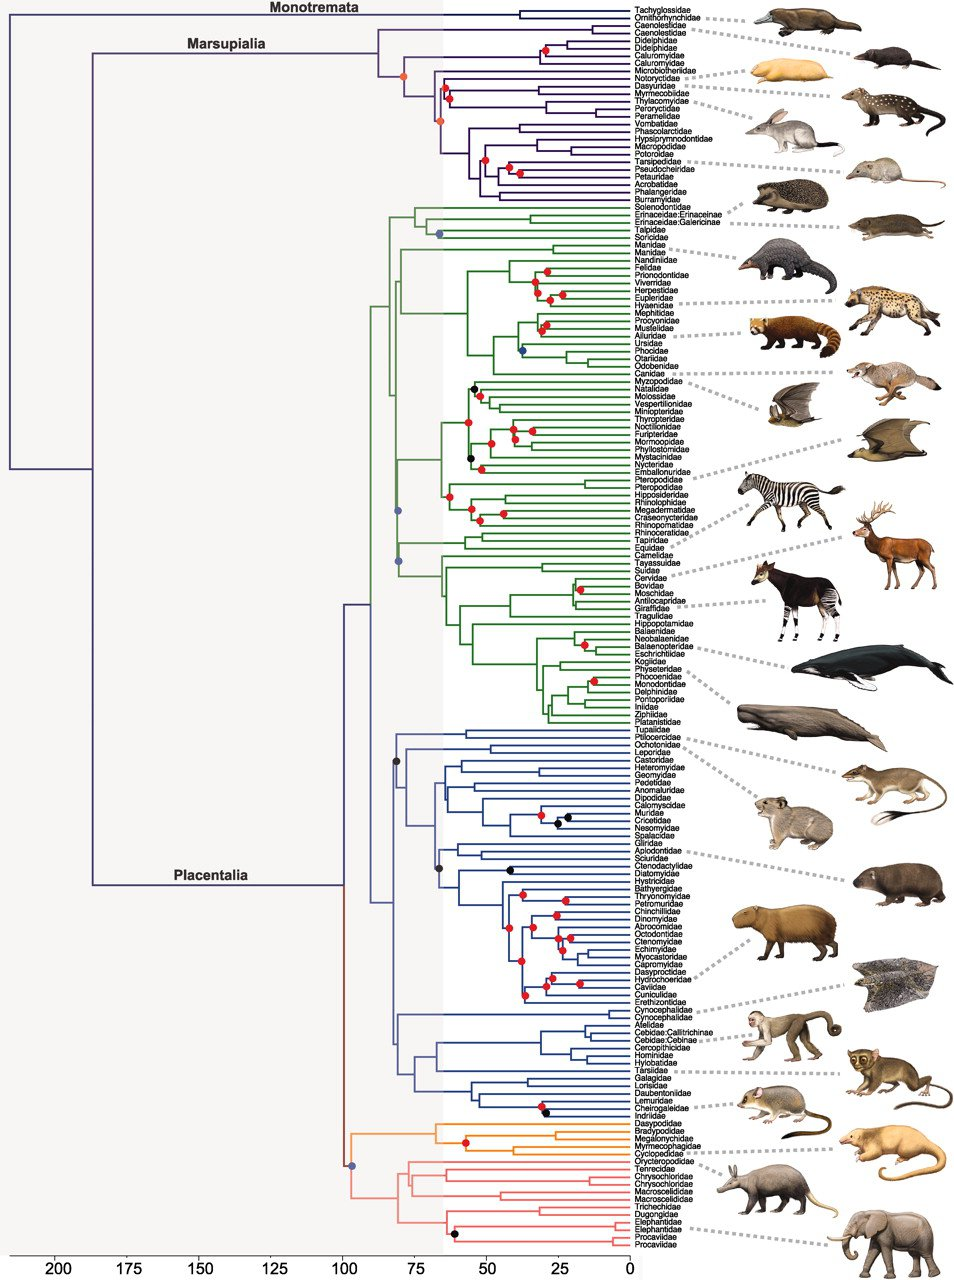
\includegraphics[width=4.5in]{../Figures/phylogeny.jpg}
\end{frame}

\begin{frame}[t]{Examples: Super Pixels}
\center
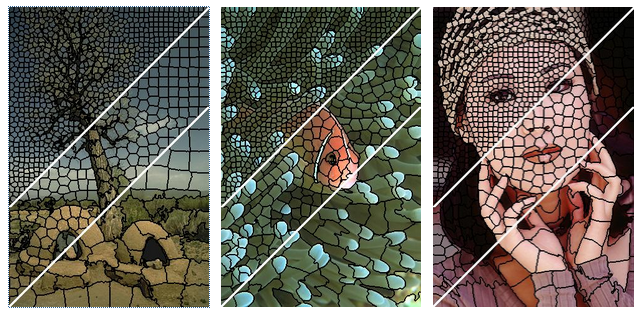
\includegraphics[width=4in]{../Figures/super_pixels.png}
\end{frame}


\section{Exhaustive Clustering}
\subsection{foo}
 
\begin{frame}[t]{Defining a Clustering}
 
\begin{itemize}
\item Suppose we have $N$ data cases $\mathcal{D}=\{\mbf{x}_i\}_{i=1:N}$.
 
 \pause \item A clustering of the $N$ cases into $K$ clusters is a partitioning 
 of $\mathcal{D}$ into $K$ mutually disjoint subsets 
 $\mathcal{C}=\{C_1,...,C_K\}$ such that 
 $C_1 \cup ... \cup C_K = \mathcal{D}$.
 
\end{itemize} 
\end{frame}

\begin{frame}[t]{Exhaustive Clustering}
 \begin{itemize}
 \item Suppose we have a function $f(\mathcal{C})$ that takes a partitioning 
 $\mathcal{C}$ of the data set $D$ and returns a score with lower scores 
 indicating better clusterings.
 
 \pause\item The optimal clustering according to $f$ is simply given by 
 $$\arg\min_{\mathcal{C}} \;\;f(\mathcal{C})$$
 
 \pause\item \textbf{Question:} What is the complexity of exhaustive clustering?
\end{itemize} 
\end{frame}

\begin{frame}[t]{Number of Clusterings}

\begin{itemize}

 \item The total number of clusterings of a set of $N$ elements is the 
Bell number $B_N$ where $B_0=1$ and $B_{n+1} = \sum_{k=0}^n {n \choose k} B_k$.

\pause \item The first few Bell numbers are: 1, 1, 2, 5, 15, 52, 203, 877, 
4140, 21147, 115975, 678570, 4213597, 27644437, 190899322, ...

\pause \item The complexity of exhaustive clustering scales with $B_N$ and is 
thus computationally totally intractable for general scoring functions. 

\pause\item We will need either approximation algorithms or scoring functions 
with special properties. 
\end{itemize}

\end{frame}

\section{Hierarchical Clustering}
\subsection{foo}

\begin{frame}[t]{Hierarchical Agglomerative Clustering}

\begin{itemize}
\item Hierarchical Clustering methods are a family of greedy tree-based 
clustering methods.

\pause\item Hierarchical Agglomerative Clustering (HAC)  is the most popular 
member of this family.

\pause\item It begins with all data cases assigned to their own clusters, and 
then greedily and recursively merges the pair of clusters that is optimal with 
respect to a given criteria.

\end{itemize}

\end{frame}

\begin{frame}[t]{Distance and Linkage Functions}

\begin{itemize}
\item Like KNN, HAC need to be supplied with a function for computing the 
distance between two data cases. This is often taken to be Euclidean 
distance, but could be any distance function.

\pause\item To merge clusters, HAC also needs what is called a linkage function 
for measuring the distance between clusters. 

\pause\item Linkage functions can differ 
significantly in their computational complexity and the clusterings they 
produce.
\end{itemize}

\end{frame}

\begin{frame}[t]{Examples of Linkage Functions}
\center
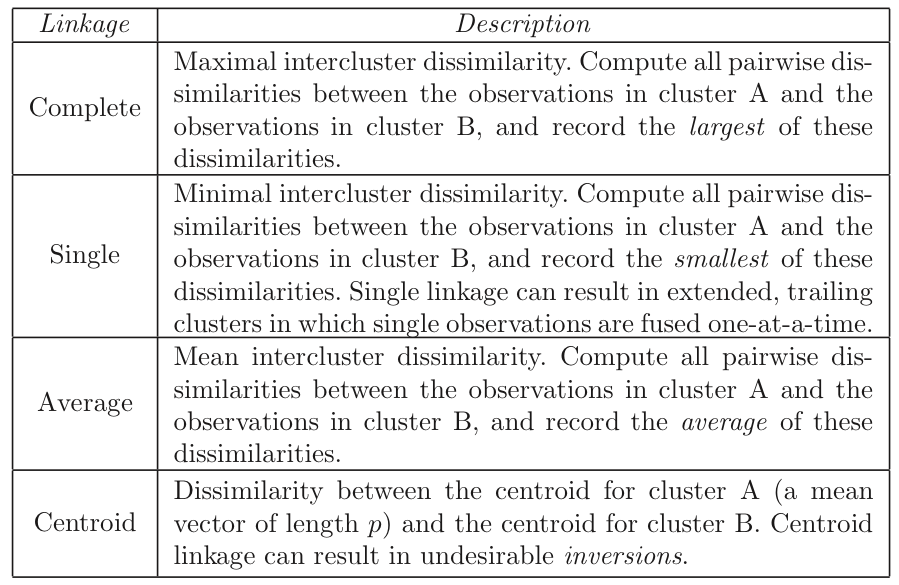
\includegraphics[width=4in]{../Figures/linkage.png}
\end{frame}


\begin{frame}[t]{The Hierarchical Agglomerative Clustering Algorithm}
\center
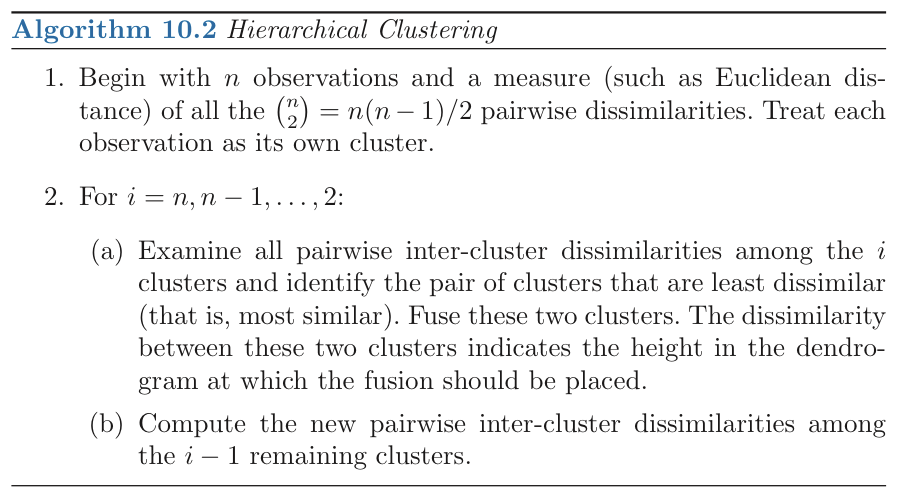
\includegraphics[width=4in]{../Figures/hac_algorithm.png}
\end{frame}

\begin{frame}[t]{Example: Data}
\center
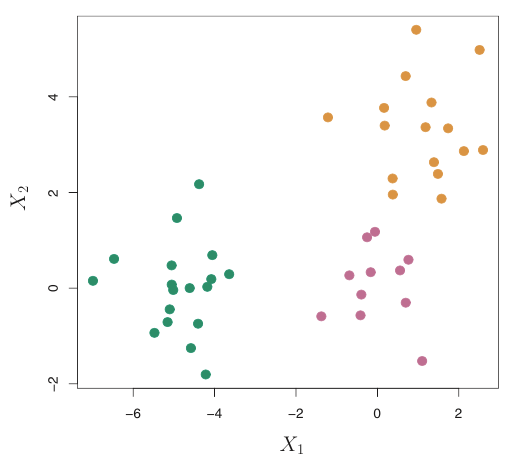
\includegraphics[width=3in]{../Figures/hac_example_data.png}
\end{frame}

\begin{frame}[t]{Example: Dendrograms}
\center
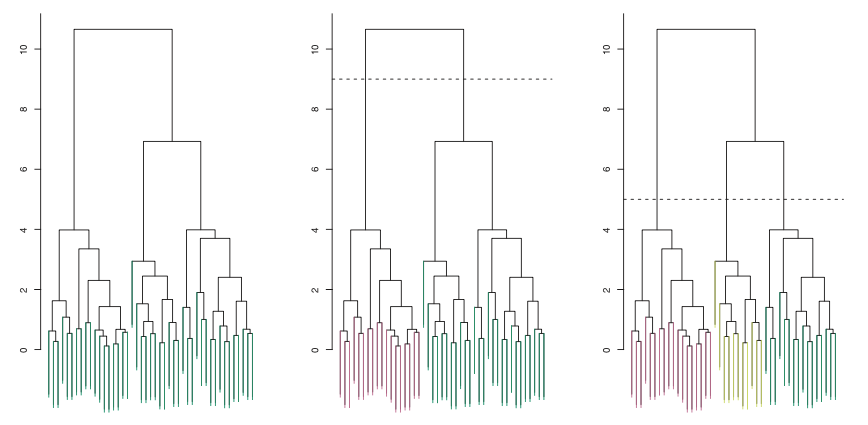
\includegraphics[width=4in]{../Figures/hac_example.png}
\end{frame}

\begin{frame}[t]{Issues}

\begin{itemize}
\item We need to have a good notion of similarity for the results of cluster 
analysis to be meaningful at all.

\pause\item As with KNN, pre-processing like re-scaling/normalizing features can
completely change the results. 

\pause\item Further, we need to slect between the different linkage functions.

\pause\item We need some way to determine the ``right'' number of clusters to 
focus on. We want to cluster on salient differences between data cases, not 
noise.

\pause \item This procedure is not able to nicely handle noise observations 
that are different from each other and from the rest of the data that do 
belong to valid clusters.

\pause \item All of these issues mean we need to be cautious in interpreting 
the results of clustering. It should  be the starting point for an exploratory 
data analysis, not the end point. 

\end{itemize}
\end{frame}




\end{document}
